%\addcontentsline{toc}{chapter}{Development Process}
\chapter{Design}\label{chap:design}

Game design has evolved a lot over the past few decades, taking advantage of more powerful devices and advances in programming generally. Game programmers were quick to take up the object-oriented banner, and were quick to become aware of its issues as well, eventually finding replacement patterns that solved the problems they came across.

There are a lot of frameworks and pre-made game engines around that allow a user to quickly get up and running in making their own games by handling the complicated parts such as rendering and input handling, asking the game designer to simply add some logic and art assets. However, these frameworks can have issues when you attempt to make a game that does not fit their predefined notions, and a lot of time could be spent hacking around their limitations to create an unusual game type.

Although it is extra work, implementing the game engine yourself gives you a lot of freedom in deciding what is necessary and what is not. Unusual aspects of the game design---such as a mix between real-time and turn-based interaction---can be accounted for and designed into the game engine much more easily, without having to first delve into unfamiliar code. This project also had the intention of learning by implementing these more technical aspects of the game engine, rather than to make a polished game on top of something that already existed.

This chapter will discuss the languages and frameworks that were used to implement the game and its engine, followed by the design of the engine itself, offering a higher level overview of the architecture as well as a more detailed look into the individual components that make up the game engine and how they fit together.

\section{Languages and Tools}
Even ignoring the direct specification of languages and technologies that the project required, the need for it to be run in a browser already limited the choice of languages and tools available to develop the game engine in.

\subsection{Languages}
\subsubsection{Client-Side}
Previously, the most popular and obvious choice for browser-based development of serious applications was ActionScript, the language that runs in Adobe's Flash plugin. This language has a lot of advantages over JavaScript---which is the language specified and the other main option---primarily in its traditional object-oriented style as well as the use of static types. Both of these are useful for creating large applications in general, but the classical object-oriented style is especially useful in game programming, as most standard patterns used in game programming were invented for languages using it; moving away from it begins to create problems of having to reinvent a lot of what has already been figured out.

ActionScript has also remained popular for creating games, despite its disappearance from other types of web application. This means that there are plenty of resources available for it, from books to libraries and frameworks.

However, despite all these advantages, ActionScript and Flash are unsuitable for this project for a few reasons. The first is ActionScript's requirement to be run in a Flash container. The project specified the use of \textsc{html5} canvas, which is a native browser construct that isn't usable by Flash, because Flash is a plugin. Its plugin status is also a potential problem for accessibility. Although it remains the most ubiquitous browser plugin for desktop use---a status most likely still conferred by its continued use for video sites like YouTube---it is an issue for mobile users who cannot install it at all, whereas a \textsc{html5} game can be run on modern mobile browsers just fine, in theory. There is also the case of it being an unfamiliar environment, particularly in regards to how to interact with the network, a problem exacerbated by the server being written in the equally unfamiliar Python.

JavaScript has the advantage of being both familiar and natively supported by browsers, letting it interact with the \textsc{html5} canvas element. Indeed, JavaScript is the only language natively supported by browsers. However, as previously mentioned, JavaScript has some disadvantages for creating games and other larger applications. While neither the lack of a more traditional object-oriented structure nor the lack of static typing make it unworkable for creating games, it does cause unnecessary issues. The lack of typing is of course the traditional (and commonly argued about) trade-off between easy prototyping and easier refactoring and debugging. The prototypal inheritance style verses the classical class structure is more of an issue, however, as all game design patterns are designed to be implemented in the latter.

The most extreme way to solve these issues is to look into languages that compile down into JavaScript while providing the features that make them more attractive to program in. Three major options exist in this area: CoffeeScript, Microsoft's TypeScript and Google's Dart.

CoffeeScript is an attempt to redo JavaScript's syntax to be more succinct, while providing some quality of life enhancements in the process. Although it does offer a way of specifying classes in the classical way, it doesn't offer typing, optional or otherwise. It is probably the most popular of the options, having been available for the longest, but has the disadvantage of needing to learn its syntax, whether that syntax is better than JavaScript's or not.

TypeScript is a superset of JavaScript, and regular JavaScript code is perfectly valid TypeScript code. This immediately gives TypeScript an advantage because it is already familiar. On top of JavaScript it adds classes and optional types---both the major features missing that are useful for game development.

Finally, Dart is a language that is intended as a complete replacement for JavaScript, even offering a native VM to run it within some experimental versions of the Chromium browser, though it can compile down to JavaScript as well. It offers many of the advantages of TypeScript, but with CoffeeScript's disadvantage of unfamiliarity.

All three languages also have the disadvantage of adding an extra compilation step, and potentially problems in making sure that the compiled code is actually sent to the browser, especially from the unfamiliar Python language and framework used on the server-side.

TypeScript was the most tempting option but was ultimately rejected because, although it is familiar in many ways, the extra steps and tooling surrounding it were considered potential issues and there was a lack of desire to add too many unfamiliar parts to the development process when the server-side would be entirely alien.

Although these options were rejected, at least one of JavaScript's problems was able to be worked around. JavaScript's prototypal inheritance style can be coerced into looking like a more classical class structure, and to that end a library known as \texttt{class.js} \cite{citeulike:13160361} was selected that implemented this. Although the library cannot deal with JavaScript's other issues, such as a lack of easy scoping inside a class or the lack of types, it created an environment that was much easier to work with when implementing the common game design patterns.

\subsubsection{Server-Side}
The project specification demanded that Python be used as the server-side language, due to a desire to to gain experience in it. The main reason for this is that it is a very popular language and is used in a lot of areas, from major science to simple scripting. It is also popular in games, acting either as a scripting language embedded into C++ code, or as the entire game engine itself. Indeed, several frameworks and game engines exist in the Python world that are designed to make games programming easier\cite{citeulike:13160372}, offering support for interacting with common graphics libraries like OpenGL, and UI libraries like Qt\cite{citeulike:13160375}.

Python is also somewhat popular in the world of web applications, offering frameworks and libraries to handle many types of networking situations, including HTTP and websockets as used in this project. However, it is certainly not the most popular language, and in some regards lags behind others in this area, particular as web development is a very fast moving world.

If Python had not been required, Node.js would likely be the choice of language for the server-side in this project. Although it is not as popular as Python in terms of the number of sites actually using it \cite{citeulike:13160383}, it has been steadily gaining traction in the web development world and a lot of modern tools and frameworks in this area are created for it and other trending languages over Python. The SocketIO library used in this project to implement websockets was made originally for Node.js, for instance.

Node.js also has the major advantage of being JavaScript, which means that it is not only familiar, but almost entirely the same as the client-side. Not having to switch languages when developing across the client and server is a definite advantage and, though it also has JavaScript's weaknesses, both CoffeeScript and TypeScript can be used instead if the language replacement route is being taken.

\subsection{Frameworks and Libraries}
Not many frameworks or libraries were used in this project, but there were some. On the client-side the \texttt{class.js} library \cite{citeulike:13160361} has already been mentioned. This allowed for a more traditional object-oriented class style when writing JavaScript, instead of JavaScript's own prototypal style.

The other library used on the client-side was one that implemented the A* pathfinding algorithm \cite{citeulike:13160393}. The decision to use this library over implementing it directly was because it was already well made and included some useful optimisations. This saves a lot of time compared to custom implementing it just for the project.

Across both server and client the library SocketIO was used, which is a more powerful implementation of the websocket technology that came about in \textsc{html5}. On the client this was used directly, as by default it is a JavaScript library. On the server-side a plugin for the Python framework chosen was used instead \cite{citeulike:13160395}.

The Python framework mentioned above is Flask \cite{citeulike:13160396}. Flask is a minimal framework for Python that provides basic features for a web application server, such as routing and rendering of templates to send to the client. Additional functionality is added in through plugins, such as the aforementioned SocketIO plugin to provide websockets and a plugin to provide easy database access.

Beyond these few things, all code was custom written.

\subsection{Database}
Most modern game designs offer the saving of state to the user. This can be achieved in a lot of ways, depending on the needs of the game. For a single-player game, it may be reasonable to save the game's state in the user's client-side storage offered by their browser, for example.

However, in a multiplayer game the server needs to keep track of everything, and there is also potentially more state to keep track of. Because of this a database is required.

The database implementation used in this project is SQLite, which stores the database in a single file and requires little set up to get running. Although it lacks many advanced features of some of the other databases available it offered enough for this project to run well. Its only disadvantage relevant to this project is that it is not as fast as something like MySQL \cite{citeulike:13160403}. However, because of the use of a Python framework to manage the database, swapping out which one is used is a case of changing only a few lines of code. This means that, should SQLite ever become a bottleneck for the game---which is unlikely---upgrades are easily implementable.

\section{Overall Architecture}
The overall architecture of a game is very important to making sure that features can be added and changed easily. A common example in the game world is that of heavy use of traditional object-oriented inheritance, where there is a very deep hierarchy. Having a few simple types of object in the world makes this manageable, but the moment you start wanting to add a lot of other different types, or special versions of something, you end up with a mess that's very hard to get out of.

The solution to this is what is known as a Component-Entity System. In this model you have generic entities that are made up of lots of individual components that each have separate functionality. In this way you can easily create a lot of different types of objects without having the mess of inheritance that the more traditional model creates. The advantage of all this abstraction is counterbalanced by vastly increased complexity in implementation. Because every part of the functionality of an entity is compartmentalised, you end up needing extra managers to handle that.

Because the game in this project was going to be very simple, with the minimal system having only two types of entity, it was decided that the Component-Entity style was not worth the extra development effort; there is only a base entity and a character type entity which inherits from it, though there is a small concession to the idea of Component-Entity on the client-side, which will be discussed in Section \ref{entities_design}.

Before getting to the details of each part, an overview is necessary to give context to their purposes. There are only a few individual components to the whole system, though they all have need to interact.

\begin{figure}
	\centering
	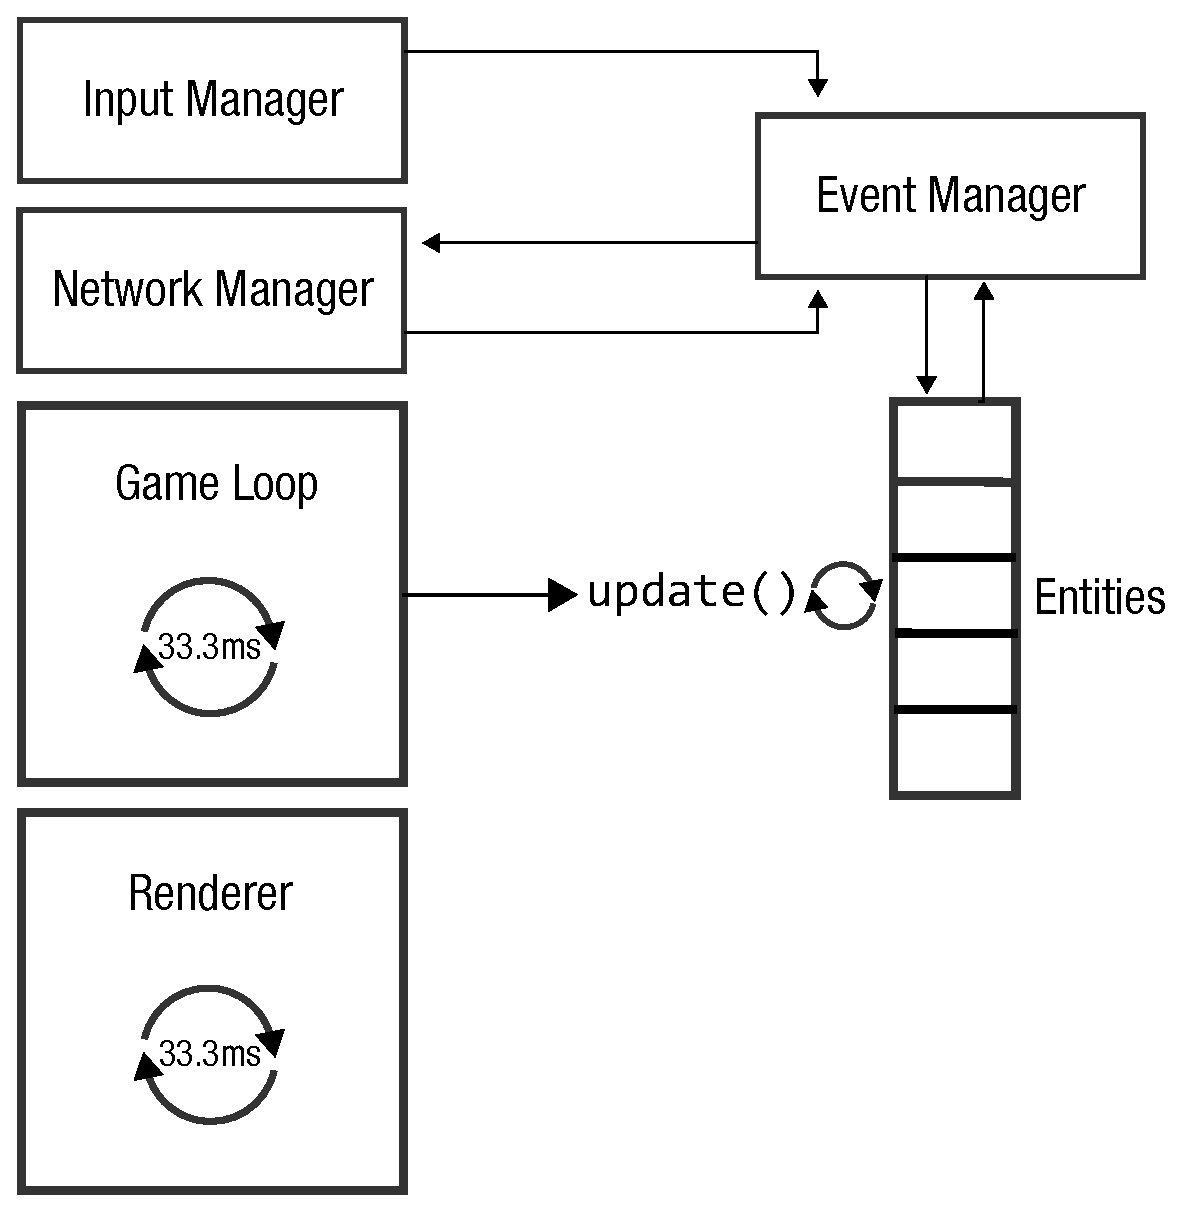
\includegraphics[width=8cm]{Images/overall_architecture.eps}
	\caption{The overall architecture of the game engine.}
    \label{fig:architecture}
\end{figure}

The most important component in the engine is the game loop. This is responsible for the updating of the game simulation every frame by asking each entity it knows about to update itself in turn. When asked to update themselves, the entities check their event queues for any new events and process them as required, then proceed to perform any necessary updates to their state, such as movement, as well as creating their own event to inform the server if relevant. These events are passed around the system by an event manager, which sits outside of the game loop. Any part of the system that wants to know about something registers itself to receive event updates related to that thing and is then given them the moment the event comes in. Finally, there is an input manager and a network manager, which handle input (and output in the case of the network manager) from players and the server.

This architecture applies fully to the client but the server makes some changes. These changes come about primarily due to implementation details and the differences between JavaScript and Python. However, the biggest difference by purposeful design is that the server needs to handle multiple games running simultaneously but apart, rather than having to deal with only one. This means that the server has a higher level manager responsible for creating games and routing messages to and from the server-side games and the clients.

% TODO: DIAGRAMS

\section{Detailed Design}

\subsection{\texttt{Engine} and \texttt{Scene}}
The \texttt{Engine} class is the central class in the game. It manages the creation of all other system classes, including the event manager, the network and input managers and the renderer, and contains the central game loop. Once the game is loaded it tells the server that the client is ready so that it can be registered to receive network events. It is also responsible for creating and giving access to the \textsc{html5} canvas used to render the game.

The \texttt{Scene} class is what describes the actual content of the game simulation at that moment. Each scene represents the map the players are currently on, and contains the terrain as well as all the entities. When the game simulation is updated, it is the entities in the \texttt{Scene} class that are affected.

To load the scene from the server, the \texttt{Scene} class contains several methods that first communicate with the server and then handle the result. The server keeps track of which scene is the currently active one in a game, so \texttt{Scene} gives the server its game ID and is given back the scene data in response. This data is processed and turned into actual terrain and entities. No other part of the game is able to create new entities.

The \texttt{Scene} class also remains the only place where the new event manager was not implemented. Due to the issues with the previous event management system, discussed in section \ref{subsection:eventmanager}, network connectivity had to be implemented directly into \texttt{Scene}, rather than abstracted to the correct \texttt{Network} class. With the event manager, this shouldn't be necessary, but the retrofitting work was not completed in this case.

\subsection{Game Loop}

\begin{figure}[H]
	\centering
	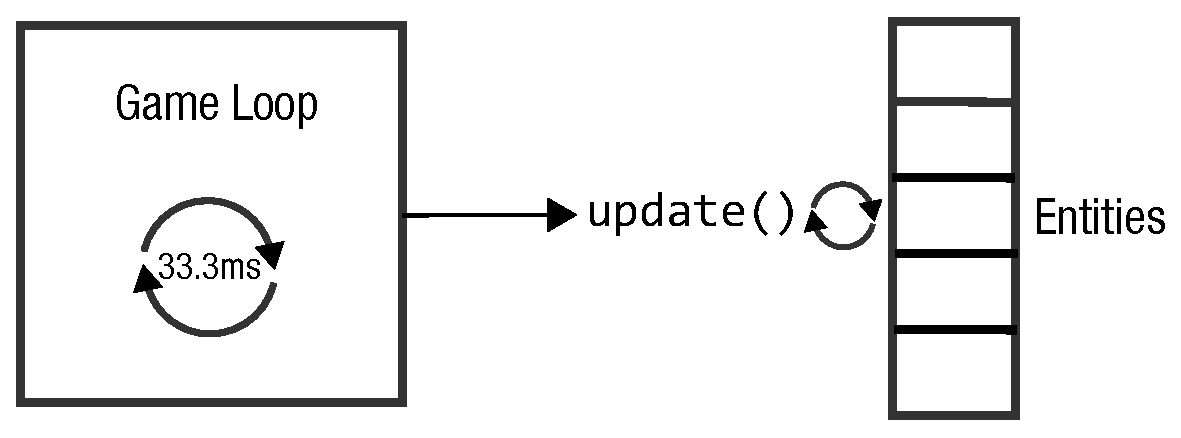
\includegraphics[width=8cm]{Images/game_loop.eps}
	\caption{The game loop updating.}
    \label{fig:gameloop}
\end{figure}

The central part of any game is what is known as the game loop. It is run from the main \texttt{Engine} class and is responsible for managing the entirety of the game, making sure every other part of it runs when it is supposed to.

An important concept to understanding the purpose of the game loop is the \textbf{frame.} This is a slice of time in the game world, with the amount of time each frame represents being decided by how many frames you wish to have per second. Common numbers chosen here are 30 and 60, meaning a frame is 33.3 milliseconds and 16.7 milliseconds respectively. While it is usually trivial to have a simple game running at 60 frames per second, it isn't always the right choice. More frames per second means more processor time used, which drains more power or could cause issues on weak devices. For this project it is also unnecessary, as the game world does not require a simulation at that level of fidelity. 30 frames per second was chosen as a good balance between smoothness of gameplay (such as moving around) and demands on power.

The purpose of the game loop is to update the simulation every frame while keeping track of whether the simulation is running at the correct speed. Every time it runs it first needs to check how much time has passed since the last frame was processed. If, for some reason, a frame took too long to process the last time then the next update will run as many times as necessary to catch back up to where it should be, regardless of whether that means things are moving too quickly in real-time or not.

The game loop itself is not directly responsible for updating the simulation, however. Rather, it calls every entity that is currently active and asks it to update itself. Once all entities have updated themselves, the network manager is asked to inform the server of everything that happened it might need to know about and the frame is complete.

\subsection{Entities}\label{entities_design}
Entities are the next most important part of the game architecture, alongside the event manager, which will be discussed next. Each entity is an object in the game world. In the Component-Entity System mentioned previously, it would be made up of many individual components, linked to a component manager so that they could talk to each other and share necessary state. The entity itself would have no real idea about what it is or what it does, simply getting each component to do something in turn, in a way similar to the game loop asking the entity to update in the first place.

However, because implementing this is very complicated, entities in the project game don't work this way. Instead, they are more traditional objects, with methods and properties. This works fine because there are only two types of entity in the game: a basic \texttt{Entity} and a \texttt{Character}.

The basic \texttt{Entity} class is a simple object in the game world like a wall. It has no properties beyond its size, position and the sprite that represents it if one exists. A \texttt{Character} is a lot more complicated, and has methods for handling user input and updating its position, as well as dealing with any other interactions that might occur, such as taking damage from another entity.

When an entity is asked to update itself, it checks the list of events that it has received from the event manager since the last update and runs through them, applying a series of functions in order. Once it is done the game loop asks the next entity along to do the same thing. Basic entities don't do anything on an update, whereas \texttt{Character}s will check for input from a player or the server and update their positions or perform an action.

The existence of two types of player with different capabilities created some issues. Initially there was actually a third entity type that inherited from \texttt{Character}, called \texttt{Player}. The \texttt{Player} class had extra functionality to find paths for itself, and interpreted player input but not server input. However, because a Game Master needs to be able to change which entity they are controlling, the \texttt{Player} class was merged with \texttt{Character} and a method for swapping between them was created.

As there were two ways to interpret any input events, and they needed to be switched out, two functions were made into components: input handling and path finding. The input handler for an active player listens for events from the input manager, whereas the input handler for a remote player listens for network events. The pathfinding component on an active player actually creates paths, whereas the remote entities simply get given them from the network.

\subsection{Event Manager}\label{subsection:eventmanager}

\begin{figure}[H]
	\centering
	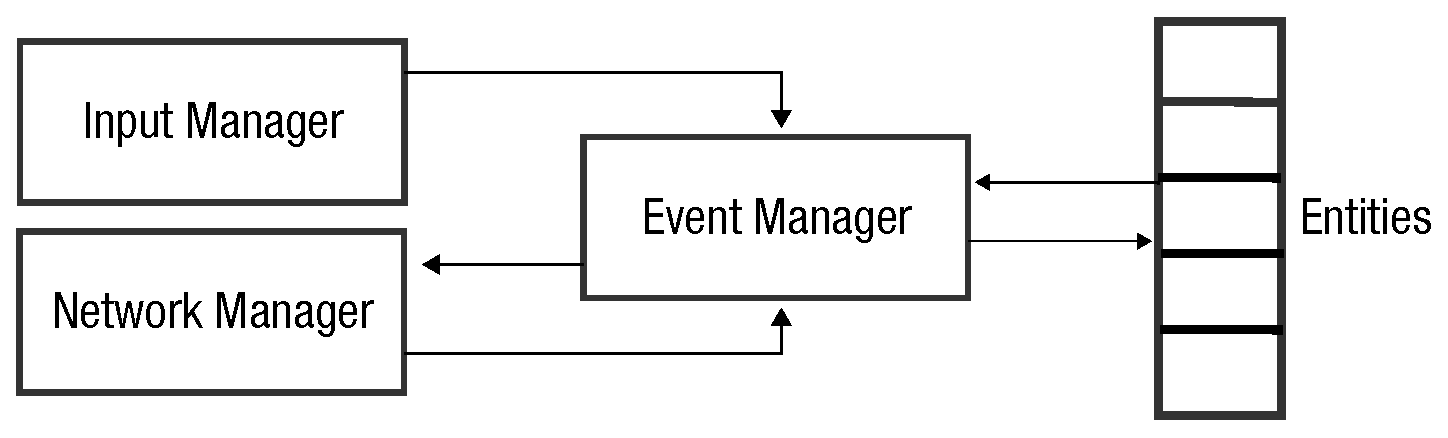
\includegraphics[width=8cm]{Images/event_manager.eps}
	\caption{The event manager.}
    \label{fig:event_manager}
\end{figure}

The event manager is an important piece of the game engine, and is the communication method for all the other system components, acting as a sort of glue between them.

Unlike almost all the other parts of the game, the event manager is not run per frame or controlled by the game loop. Rather, it receives and propagates events as it gets them. This means that events that are created in the middle of a frame's update are still sent to the things that need them.

This has some advantages. The main advantage is network latency. Because the network latency is several frames long, the ability to have the network send events back in the same frame that they happen helps to reduce any time wasted. Another small time-saver in this regard is that an entity affecting another entity may be able to have that effect be known about in the same frame, as long as the acting entity is processed before the entity being acted upon. In the case of an affected entity being updated first, however, it will only take into account the new information in the next frame. This isn't a huge issue, and a user should never really notice that something has happened one frame after, but the inconsistency is there and could potentially cause problems in situations where frames are taking a long time to process.

Despite the seeming obviousness of its use, the event manager originally didn't exist, and input was handled by having a single event queue stored in the \texttt{Engine} class. This event queue was given to entities from the update call in the game loop and they ran over each event looking for something relevant to them. It was also very difficult for entities to put anything into the event queue themselves, such as network input. Because of this, network events were created directly. Worst of all, because there was no way to know whether events were handled, the entire event queue was cleared on each frame, which meant that no events could be carried over.

Obviously this approach had several disadvantages. Firstly it was inefficient. Although generally there was only going to be one or two events in any given frame, there are potentially a lot of entities that have no interest in events that are stored in the event queue, so having them loop over those events is useless. Secondly, in order to update the network or add anything back into the event queue, entities had to be given the network and engine objects and pass them around. The emptying of the entire queue also meant that in situations where one entity wanted to affect another but was updated after the entity it was affecting, the affected entity would never know about it.

Replacing this system with a proper global event manager allowed for entities to no longer care about events that don't matter to them, as well as much more easily carry over events from frame to frame, even leaving events unhandled for a long time if necessary. Unfortunately the refactoring to use the event manager wasn't entirely completed, as seen with the previously mentioned \texttt{Scene} class. However, the vast majority of the game uses it.

\subsection{Renderer}\label{design_renderer}
The renderer is responsible for displaying frames to the player, acting as the view into the simulation. It is also another part of the game engine that is separated from the game loop. It isn't required for this to be the case in order for the game to function; indeed, with the simplicity of the game in this project the renderer could be tied to the game loop's frames pretty easily and cause no problems. It is, however, considered to be good practice to separate them, and for good reason. The renderer is almost always the most taxing part of the whole game. By adding the renderer to the central game loop's update process you cause each frame in the simulation to take a lot longer to complete. If this addition doesn't cause the frame to run over time then no problems will be noticed. Unfortunately, it is very easy for the renderer to cause frames to run over time and, if it happens consistently, the game loop could get stuck in an infinite loop attempting to catch up.

By separating the renderer out, you can make sure that the central game loop always updates correctly and keep the simulation running, regardless of how many frames the renderer is managing to actually display to the user. It is desirable to make sure that the renderer is managing to display all the frames, but it's less of a problem if the renderer can only display 20 of them than it is to have the central game loop stuck trying to catch up.

The renderer does not render the world in one go. Rather, it renders the terrain first, and then renders entities on top of it. The reason for this is one of efficiency. The terrain never moves and never crosses tile boundaries. It also comes pre-ordered in a grid. These attributes make it easy to render by simply drawing each tile to the screen one by one in order. Entities, however, can have different heights and can move around and cross tile boundaries, which requires that they get sorted properly, creating rendering overhead. By rendering the terrain first, there is less that needs sorting afterwards, thus speeding up the renderer.

\subsection{Input Manager}
A game isn't much of a game if the user cannot create any input. To handle the user's input there is an input manager, which is responsible for capturing all of a player's input, working out what purpose that input has and then creating an event for it in the event manager, which propagates it to all interested parties.

The input manager is only able to work out what user input means, not what that input applies to. In other words, it knows that a user clicking means the user wants to move somewhere, checks that it is a valid input and then creates an event to say that there has been a movement input and the tile to move to. This event is passed to all entities that subscribe to movement events and it is up to them to work out whether it is relevant or not.

\subsection{Network}
The \texttt{Network} class is responsible for managing the connection the game has to the server. At the end of every frame it will inform the server of anything the client's player has done, such as moved his character to a new location.

If the server sends a message, however, the network manager will immediately create an event for it. Although this is mostly due to technical implementation reasons, there are advantages in this. Primarily, it means that entities being affected by network events can be updated sooner as they don't necessarily have to wait till the next frame. This is important for the same reason as the event manager, by reducing latency from a very high latency aspect of the game.

\subsection{Server Differences}
%todo: add diagrams here explaining the server architecture

\begin{figure}[H]
	\centering
	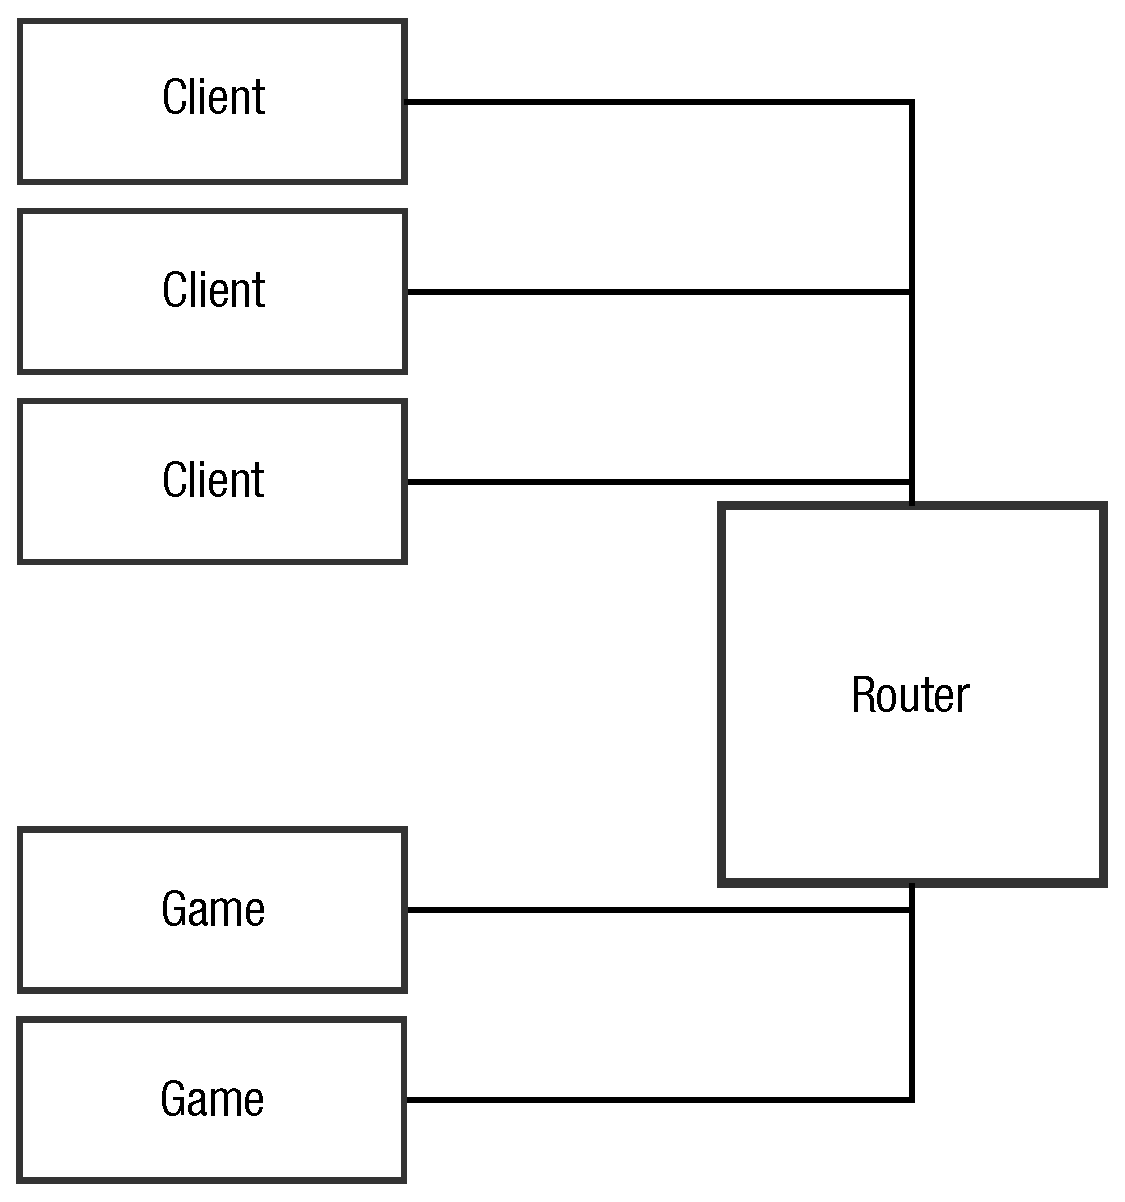
\includegraphics[width=8cm]{Images/server_design.eps}
	\caption{The server contains the router and some games. The clients interact with the game they are interested in through the router.}
    \label{fig:server_design}
\end{figure}


The server's purpose is to act as a central version of the game that links all the clients together, and is responsible for being something of an authority in the game simulation to make sure that clients see the correct things. Because of this it makes sense that the server and client have the same structure.

However, there are, in fact, differences between them. The reason for this is entirely due to implementation---which will be discussed in more detail in the next chapter---but regardless of the reasons it's important to understand these differences.

The most important and major difference is that the server runs many games simultaneously, rather than just a single game at a time. To handle this, a higher level is needed to manage the games and route messages to and from players. The router that handles this is a traditional web application router, made using the Flask framework. It takes incoming HTTP connections and works out what they are supposed to do based on the URL. Once a game is up and running and users are connected, they communicate with it through the SocketIO library providing websockets, which the router also manages.

Each game itself is run in a separate thread, providing an architecture as similar to the one in the client as possible. Communication between the router and any individual game is handled through thread-safe queues, as it is impossible to call a method in the thread directly due to the game loop blocking and taking control.

The game loop itself is probably the most major difference in the internal game architecture, entirely by way of implementation details. The client's JavaScript version of the game loop is essentially non-blocking as it has to always yield control back to the browser. However, Python has no native way of achieving this style---known as an event loop---and the libraries available to implement it are complicated. Because of this, the Python implementation of the game loop is a more traditional \texttt{while} loop, running until a flag indicating the game is to be shut down is set to false.

Although this does not affect the fundamental way of updating entities, which is the bulk of the work the game simulation performs on the server, other aspects of the architecture are changed because of it.

There is no proper event manager in the style that was added to the client, as there is no easy way for it to be run outside of the game loop without creating another separate thread for it---an undesirable option for a server that will already be having to manage many of them. Because of this, the server event management remains in the original style that the client had before the event manager was implemented: the game loop contains a data structure that stores all the events and asks the entities to take a look at them in turn and see whether they care.

In a concession to sanity, however, the server uses a queue to store input events (accessible by the router so that they can be passed in) and doesn't delete unhandled events at the end of every frame. Output is placed into another queue that the router can check in order to inform clients of anything interesting.

Other parts of the architecture are simply removed: there is no renderer because the server's view is entirely remote---no one is ever going to be trying to play the game on the server directly. The server also doesn't have an input manager for the same reason. The network manager is pushed up into the router, rather than being a special part of the game engine.

This design is, of course, not perfect. The biggest issue is one of scalability. This model works fine for one or two games running at once, but because the router has to manage connections for all active games it can very quickly get overloaded, especially when players decide to spam actions that create network events such as movement commands.

Ideally each game would be responsible for handling its own connections and the router would simply exist to get players connected to the right game. This creates independence of the router and game servers and is a much more scalable solution. The reason it doesn't do this, however, is just because the implementation knowledge necessary for this was not available and time did not allow for further investigation into it. A less than ideal working solution was considered to be the better choice than potentially having no solution at all because the implementation was too hard given skill, knowledge and time available.

% The game simulation running on the server operates with the same fundamental architecture, with the exception of having no input manager as there can never be any direct input to the server. However, because the server has to operate many games at once, there is another level higher than the client-side has.

% The server has a traditional web application router that receives and routes events from the client. These events are things like joining or leaving a game as well as the things a client cares about like movement. In this way, it takes the place of the \texttt{Network} class in the client.

% Each individual game is run in a separate thread due to the blocking nature of the game loop. The server keeps track of who is connected to what game and sends events that are relevant to a game to that game alone, which means that there is no pointless spamming of irrelevant events to games that don't care about it.

% This higher level part of the server is also responsible for creating game threads when a user first connects to a game. However, the game loop itself is responsible for shutting itself down, though the router can ask the game to do so as well.

% You should concentrate on the more important aspects of the design. It is essential that an overview is presented before going into detail. As well as describing the design adopted it must also explain what other designs were considered and why they were rejected.

% The design should describe what you expected to do, and might also explain areas that you had to revise after some investigation.

% Typically, for an object-oriented design, the discussion will focus on the choice of objects and classes and the allocation of methods to classes. The use made of reusable components should be described and their source referenced. Particularly important decisions concerning data structures usually affect the architecture of a system and so should be described here.

% How much material you include on detailed design and implementation will depend very much on the nature of the project. It should not be padded out. Think about the significant aspects of your system. For example, describe the design of the user interface if it is a critical aspect of your system, or provide detail about methods and data structures that are not trivial. Do not spend time on long lists of trivial items and repetitive descriptions. If in doubt about what is appropriate, speak to your supervisor.

% You should also identify any support tools that you used. You should discuss your choice of implementation tools - programming language, compilers, database management system, program development environment, etc.

% Some example sub-sections may be as follows, but the specific sections are for you to define.

% \section{Overall Architecture}

% \section{Some detailed design}

% \subsection{Even more detail}

% \section{User Interface}

% \section{Other relevant sections}